\section{ نتایج و تحلیل}
{  در این بخش ابتدا روش ارزیابی مورد استفاده در این مسئله را بررسی می‌کنیم. سپس به این موضوع می‌پردازیم که مشکل بیش برازش در اینجا چگونه تعریف می‌شود و برای حل آن باید چه کارهایی انجام دهیم. در نهایت نتایج هر کدام از روش‌ها را بررسی خواهیم کرد. دقت شود که در برخی از جدول‌ها از اصلاح hard‌ و soft استفاده شده است. که hard به معنای این است که 
	 \lr{Early stopping}
	  بر اساس خطای داده‌های ارزیابی است و در این حالت مدل حداکثر قدرت خود نخواهد رسید. soft به این معنی است که 
	  \lr{Early stopping}
	  براساس دقت داده‌های ارزیابی است و مدل به حداکثر قدرت خود خواهید رسید. کدهای پروژه را می‌توانید در
	  \href{https://github.com/maryamhashemi/Persian_VQA}{ گیت هاب}
	  مشاهده کنید.
	\subsection{پروتکل ارزیابی}
	{
		در مقاله
		\cite{antol2015vqa}
		، معیار ارزیابی خاصی برای این مساله استفاده شده است. به عبارتی دقت را مانند روش‌های معمول در یادگیری ماشین محاسبه نمی‌کنیم. برای محاسبه دقت ارزیابی پاسخ‌های تولید شده برای سوال (نه انتخاب از بین پاسخ‌های چند گزینه‌ای)   درمجموعه مورد ارزیابی، فرمول زیر را داریم :
		\begin{equation}
		accuracy = min(\frac{\# humans that provided that answer}{3} , 1)
		\label{eq:2}
		\end{equation}
		در مجموعه‌داده اصلی برای داده‌های آموزش و ارزیابی، به ازای هر سوال 10 پاسخ انسانی گردآوری شده است که افراد مختلف به آن سوال با سطوح اطمینان مختلف، پاسخ داده‌اند. حال با توجه به این‌که ما مدل را بر روی مجموعه آموزش، آموزش داده‌ایم و بر روی مجموعه ارزیابی، آن را مورد ارزیابی قرار می‌دهیم، دقت را از این طریق محاسبه می‌کنیم.
		
		طبق این فرمول برای این‌که پاسخ پیش‌بینی شده توسط ماشین به یک سوال کاملا صحیح در نظر گرفته شود، می‌بایست پاسخ ماشین، با پاسخ حداقل 3 عامل انسانی یکسان باشد و در نتیجه امتیاز کامل 1 را از ارزیابی آن سوال دریافت می‌کند. با توجه به فرمول اگر 2 نفر پاسخشان با پاسخ مدل یکی باشد، امتیاز 0.66 و اگر پاسخ مدل تنها با پاسخ یک نفر از آن 10 عامل انسانی یکسان باشد، امتیاز 0.33 دریافت می‌کند.
		
		همانطور که می‌بینیم ارزیابی سهل گیرانه تری نسبت به ارزیابی معمولی یک پاسخ (که وضعیت 0 یا صدی صحت برای آن متصور می‌شود)، معرفی شده‌است.  این روش برای ارزیابی مسئله VQA برای اولین بار در 
		\cite{antol2015vqa}
		معرفی شده است. در حال حاضر که حدود 5 سال از انتشار آن می‌گذرد، قریب به اتفاق مقالات و روش‌های دیگر در این زمینه از این فرمول برای ارزیابی روش یادگیری خود استفاده نموده‌اند و به عنوان فرمولی استاندارد و مناسب به عنوان پروتکل ارزیابی در VQA شناخته شده است.
		
	}

	\subsection{بیش برازش، زمان رخ دادن و حل آن}
	{
		در فاز پیشرفت پروژه، نتایجی که بر روی روش پایه مقاله با داده‌های کم بدست آوردیم؛ نشان از بیش برازش داشت. در این فاز بررسی‌ها و آزمایش‌های متعددی انجام دادیم تا علت مشکل و روش حل آن را بیابیم.
	مقاله
		\cite{ilievski2017simple}
		ریشه این مسئله و رواج داشتن آن به شکل کلی و معمول در VQA را بررسی کرده است.   زمانی که معیار خطا را 
		\lr{cross entropy}
		 در نظر می‌گیریم؛ به صورت سخت‌گیرانه عمل می‌کنیم زیرا اگر پاسخ مدل دقیقا برابر با پاسخ صحیح نباشد، مدل جریمه می‌شود. این در حالی است که عبارت
		\ref{eq:2}
		  از روش سهل گیرانه‌تری استفاده می‌کند. در نتیجه این امر باعث اختلاف بین معیار خطا
		\lr{cross entropy}
		و دقت  مدل می‌شود. در
	    \cite{ilievski2017simple}
		به معرفی معیار خطا
		\lr{soft cross entropy}
		  پرداخته شده است و در محاسبه خطا، تمامی پاسخ‌های انسانی را درنظر می‌گیرد که اختلاف بین رفتار loss و دقت کاهش می‌یابد و همگرایی آموزش مدل نیز بهبود می‌یابد. بنابراین معیار اصلی برای تشخیص بیش برازش، استفاده از عبارت
		  \ref{eq:2}
		 است که به عنوان پروتکل استاندارد ارزیابی در این حوزه شناخته می‌شود. 
		 \begin{figure}[H]
		 	\centering
		 	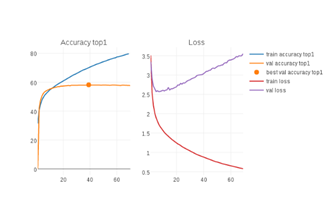
\includegraphics[scale=0.3]{images/i2.jpg}
		 	\caption{}
		 	\label{fig:9}
		 \end{figure}
		 برای مثال در شکل
		  \ref{fig:9}
		  از نظر
		  \lr{cross entropy}
		   بیش برازش داریم اما از نظر پروتکل ارزیابی بیش برازش اتفاق نیفتاده است و بهترین دقت در گام 40 رخ داده است.
		   
		   \begin{figure}[H]
		   	\centering
		   	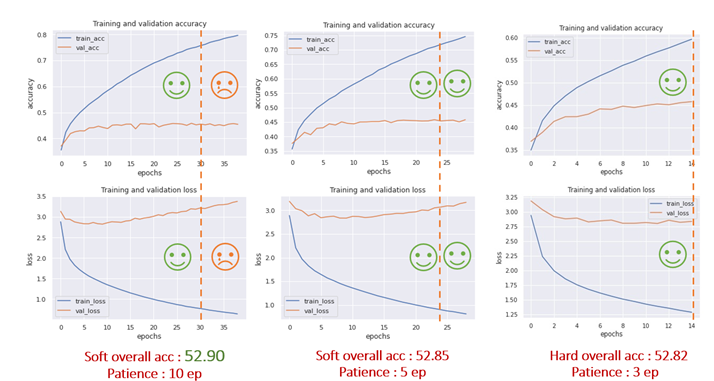
\includegraphics[scale=0.7]{images/i3.png}
		   	\caption{}
		   	\label{fig:10}
		   \end{figure}
	   
		   شکل
		   \ref{fig:10}
		  نتایج سه آزمایشی که با استفاده از 
		  \lr{Early stopping}
		   برمبنای دقت با patience های متفاوت و خطای 
		   \lr{cross entropy}
		   اجرا شده است را نشان می‌دهد. در ستون سمت راست از p برابر با 3 استفاده شده است و یادگیری در گام چهاردهم متوقف شده است. در این آزمایش از نظر خطا، بیش برازشی اتفاق نیفتاده است و به دقت
		   $ 52.82 $
		   رسیده‌ایم. در آزمایش دوم p را بیشتر کرده‌ایم و یادگیری در گام 24 به اتمام می‌رسد.از نظر تابع خطا تا گام 24 هم بیش برازش اتفاق افتاده است. اما دقت بیشتر شده است پس طبق پروتکل بیش برازشی اتفاق نیفتاده است. در ستون سوم با افزایش p یادگیری در گام 30 به پایان می‌رسد و دقت از مرحله قبل  بیشتر شده است. این نشان می‌دهد که در ستون دوم حتی بعد از گام 24 نیز بیش برازش رخ نداده است و تنها جایی که احتمالاً دچار بیش برازش اتفاق افتاده است، از گام 30 به بعد است (چرا که ممکن است اگر p را بیشتر می کردیم سناریوی آزمایش‌های قبل تکرار شود.). در نهایت  بهترین مدل در گام 30 می‌باشد.
		   
 زمانی که مشکل بیش برازش رخ می‌دهد، برای حل آن از نرمالیزه سازی l2 تصاویر، 
  \lr{recurrent dropout}
   و بهینه سازهای متفاوت مثل adam و adadelta  و یا RmsProp‌ با نرخ یادگیری کاهشی استفاده می‌کنیم.
		   
		  
		
	}
	\subsection{\lr{LSTM Q + norm I}}
	{
		آزمایش‌های متعددی برای این روش انجام شده است که جزئیات کامل آن در فایل‌های ضممیه قرار داده شده است. در اینجا به بررسی مهم‌ترین نتایج می‌پردازیم. 
		
		پس از بررسی نتایج آزمایش‌های ضمیمه شده به نتایج زیر دست یافتیم:
		\begin{enumerate}
			\item بهترین بهینه‌ساز adadelta با نرخ یادگیری 1 است که همگرایی مدل را افزایش می‌دهد.
			\item برای پیش پردازش سوال ها از کتابخانه hazm استفاده کرده‌ایم که منجر به افزایش دقت شد و همچنین روش pre در padding عملکرد بهتری از‌ حالت post‌ داشت .
			\item برای embedding سوال‌ها از fasttext‌ استفاده می‌کنیم زیرا عملکرد آن نسبت به Glove بهتر است.
			\item استفاده از \lr{recurrent dropout} به جای dropout معمولی نتایج را بهبود می‌دهد.
			\item استفاده از BatchNormalization‌ دقت‌ مدل را افزایش می‌دهد.
		\end{enumerate}
	
	نتایج این مدل را برای زبان فارسی در جدول 
	\ref{tabel:4}
	می‌توانید مشاهده کنید. در هر دو حالت سخت و نرم دقت برای ترجمه‌های Google بهتر از ترگمان است و همان طور که پیش بینی می‌کردیم دقت مدل‌های نرم بیشتر از مدل‌های سخت است و نشان می‌دهد که مدل از حداکثر ظرفیتش استفاده کرده است.
	
		\begin{table}[H]\centering
			\begin{latin}
				\begin{small}
					\begin{tabular}{ c|| c c c c || c c c c} \toprule
						\multicolumn{1}{c ||}{ }&\multicolumn{4}{c||}{\textbf{Google Translation}} & \multicolumn{4}{c}{\textbf{Targoman Translation}} \\ \midrule
						\textbf{Method} & \textbf{yes/no} & \textbf{Number} & \textbf{Other} & \textbf{All} & \textbf{yes/no} & \textbf{Number} & \textbf{Other} & \textbf{All} \\ \midrule
						\textbf{lstm Q + VGG19(hard)} & 76.14\ & 32.97\ & 35.78\ & 50.53\ & 75.58\ & 32.61\ & 33.53\ & 49.15\ \\
						\textbf{lstm Q + VGG19(soft)} & 76.74\ & 32.5\ & 36.98\ & \textbf{51.3}\ & 76.86\ & 31.85\ & 36.26\ & \textbf{50.91}\ \\
						%\textbf{lstm Q + VGG19} & \ & \ & \ & \ & \ & \ & \ & \ \\
						\bottomrule
					\end{tabular}
				\end{small}
			\end{latin}
			\caption{دقت  روش \lr{baseline} بر روی مجموعه‌داده فارسی تهیه شده.}
			\label{tabel:4}
		\end{table}
	
	همین آزمایش را برای زبان انگلیسی در دو حالت استفاده از  ویژگی‌های آماده یا ویژگی‌های تولید شده توسط خودمان اجرا کردیم. نتایج در جدول 
	\ref{tabel:5}
	آورده شده است. در حالت نرم دقت ها به دقت 
	\cite{antol2015vqa}
	بسیار نزدیک شده است. فاصله‌ی دقت‌ها در هر دو حالت نرم و سخت بین ویژگی‌های آماده و ویژگی‌هایی که ما تولید کرده‌ایم بسیار کم است و این نشان می‌دهد که توانسته‌ایم ابن بخش را تا حد خوبی به درستی پیاده‌سازی و اجرا کنیم.
		\begin{table}[H]\centering
			\begin{latin}
				\begin{small}
					\begin{tabular}{ c|| c c c c || c c c c} \toprule
						\multicolumn{1}{c ||}{ }&\multicolumn{4}{c||}{\textbf{ٍEnglish-paperToken}} & \multicolumn{4}{c}{\textbf{English-kerasToken}} \\ \midrule
						\textbf{Method} & \textbf{yes/no} & \textbf{Number} & \textbf{Other} & \textbf{All} & \textbf{yes/no} & \textbf{Number} & \textbf{Other} & \textbf{All} \\ \midrule
						\textbf{lstm Q + VGG19(hard)} & 78.43\ & 33.7\ & 37.99\ & 52.58\ & 78.53\ & 31.91\ & 38.78\ & 52.79\ \\
						\textbf{lstm Q + VGG19(soft)} & 79.34\ & 32.69\ & 40.41\ & \textbf{54.01}\ & 79.41\ & 33.62\ & 39.42\ & \textbf{53.66}\ \\
						\bottomrule
					\end{tabular}
				\end{small}
			\end{latin}
			\caption{دقت  روش \lr{baseline} بر روی مجموعه‌داده انگلیسی .}
			\label{tabel:5}
		\end{table}
	آزمایش های دیگری نیز انجام دادیم که برای استخراج ویژگی از تصویر از شبکه ی 
	\lr{resNet152}
	 و برای استخراج ویژگی از سوال از LSTM ، BiLSTM‌ و CNN‌ های یک بعدی استفاده کرده‌ایم. با توجه به جدول‌های
	 \ref{tabel:4}
	 و
	 \ref{tabel:6}
	 استفاده از 
	 \lr{resNet152}
	 به جای 
	 \lr{VGG19}
	 منجر به افزایش دقت شده است. نکته‌ی دیگر این است که استفاده از BiLSTM‌ در هر دو حالت نرم و سخت باعث کاهش دقت شده است. بنابراین بهترین مدلی که در این روش بدست می‌آید زمانی است که از ترجمه‌های Google ‌و از شبکه‌ی 
	 \lr{resNet152}
 و LSTM  استفاده کنیم که دقت
 $53.58$
 را می‌دهد.
		\begin{table}[H]\centering
			\begin{latin}
				\begin{small}
					\begin{tabular}{ c|| c c c c } \toprule
						\multicolumn{1}{c ||}{ }&\multicolumn{4}{c}{\textbf{Google Translation}}  \\ \midrule
						\textbf{Method} & \textbf{yes/no} & \textbf{Number} & \textbf{Other} & \textbf{All} \\ \midrule
						\textbf{BilstmQ+resNet152(hard)} & 76.46\ & 31.63\ & 38.6\ & 51.89\ \\
						\textbf{lstmQ+resNet152(hard)} & 76.83\ & 31.75\ & 38.77\ & 52.13\ \\ 
						\textbf{CNNQ+resNet152(hard)} & 78.34\ & 31.91\ & 38.98\ & 52.82\ \\
						\textbf{BilstmQ+resNet152(soft)} & 78.22\ & 33\ & 39.89\ & 53.37\ \\
						\textbf{lstmQ+resNet152(soft)} & 78.5\ & 31.76\ & 40.4\ & 53.58\ \\ 
						\textbf{CNNQ+resNet152(soft)} & 78.38\ & 32.36\ & 38.99\ & 52.9\ \\
						\bottomrule
					\end{tabular}
				\end{small}
			\end{latin}
			\caption{دقت  روش \lr{baseline} با استفاده از ویژگی‌های استخراج شده از شبکه ResNet152 .}
			\label{tabel:6}
		\end{table}
	
	}
	\subsection{\lr{Stacked Attention Network}}
	{
		این روش را به دو صورت آزمایش کرده‌ایم. در حالت اول برای استخراج ویژگی از سوال، از دو لایه LSTM 1024 تایی با
		 \lr{recurrent dropout}
		   با نرخ $0.5$ استفاده می‌کنیم. بعد از هر لایه‌ی LSTM‌ یک لایه‌ی BatchNormalization‌ قرار می‌دهیم. در حالت دوم برای استخراج ویژگی از سوال، از روش CNN های یک بعدی با فیلتر سایز‌های 1، 2 و 3 که به ترتیب تعداد فیلتر‌ها برای هر کدام 256، 256 و 512 است؛ استفاده می‌کنیم. در هر دو حالت آزمایش از دو لایه‌ی attention به ابعاد 1024‌‌استفاده می‌کنیم. برای پیاده‌سازی این روش از Tensorflow.keras استفاده کرده‌ایم. از Adam به عنوان بهینه‌ساز با نرخ یادگیری $0.0005$ استفاده کردیم. سایز batch‌ را برای همه‌ی آزمایش‌های این بخش 300 قرار دادیم. شبکه را با حداکثر 50‌ گام به همراه 
		  \lr{Early stopping}
		   آموزش می‌دهیم تا زمانی که خطا روی داده‌های ارزیابی در 3 گام آخر تغییر نکند.
		   
		    نتایج حاصل از این شبکه را در جدول
		\ref{tabel:1} 
		می‌توانید مشاهده کنید. همانطور که پیداست به طور کلی دقت برای حالتی که از ترجمه‌های Google استفاده می‌کنیم بیشتر است. زمانی که از ترجمه‌های Google استفاده می‌کنیم، روش  LSTM دقت بالاتری دارد اما زمانی که از ترجمه‌های ترگمان استفاده می‌کنیم دقت روش CNN بیشتر است. نکته‌ی حائز اهمیت در اینجا این است که دقت بین دو حالت LSTM‌ و CNN‌ چندان تفاوتی ندارد اما از لحاظ منابع محاسباتی روش CNN به صرفه‌تر است زیرا تعداد پارامترها در روش CNN‌ تقریبا 8 میلیون و در روش LSTM‌‌ 22 میلیون می‌باشد.‌
		\begin{table}[H]\centering
			\begin{latin}
				\begin{small}
					\begin{tabular}{ c|| c c c c || c c c c} \toprule
						\multicolumn{1}{c ||}{ }&\multicolumn{4}{c||}{\textbf{Google Translation}} & \multicolumn{4}{c}{\textbf{Targoman Translation}} \\ \midrule
						\textbf{Method} & \textbf{yes/no} & \textbf{Number} & \textbf{Other} & \textbf{All} & \textbf{yes/no} & \textbf{Number} & \textbf{Other} & \textbf{All} \\ \midrule
						\textbf{SAN\_LSTM\_2} & 77.83\ & 33.19\ & 39.08\ & 52.84\ & 75.95\ & 31.61\ & 36.82\ & 50.81\ \\ 
						\textbf{SAN\_CNN\_2} & 77.49\ & 33.17\ & 39.18\ & 52.76\ & 76.48\ & 32.29\ & 37.37\ & 51.37\ \\
						\bottomrule
					\end{tabular}
				\end{small}
			\end{latin}
			\caption{دقت  روش \lr{Stacked Attention Network}.}
			\label{tabel:1}
		\end{table}
		
		برای بررسی تاثیر تعداد لایه‌های attention ، مدل را در سه حالت که تعداد لایه‌های attention 1، 2 و 3 باشد؛ آموزش می‌دهیم. با توجه به جدول 
		\ref{tabel:2} 
		دقت وقتی تعداد لایه‌های attention 2 است بیشتر است. این نشان دهنده‌ی این است که ما برای بدست آوردن پاسخ نیاز به استدلال چند مرحله‌ای داریم. به همین خاطر یک لایه‌ی attention کافی نیست. از طرفی اگر تعداد لایه‌ها بیشتر از حدی باشد منجر به پاسخ اشتباه می‌شود. در اینجا زمانی که تعداد لایه‌ها را بیشتر از 2 قرار دهیم منجر به کاهش عملکرد مدل می‌شود.
		\begin{table}[H]\centering
			\begin{latin}
				\begin{small}
					\begin{tabular}{ c|| c c c c } \toprule
						\multicolumn{1}{c ||}{ }&\multicolumn{4}{c}{\textbf{Google Translation}}  \\ \midrule
						\textbf{Method} & \textbf{yes/no} & \textbf{Number} & \textbf{Other} & \textbf{All} \\ \midrule
						\textbf{SAN\_LSTM\_1} & 77.46\ & 32.23\ & 38.35\ & 52.22\ \\
						\textbf{SAN\_LSTM\_2} & 77.83\ & 33.19\ & 39.08\ & 52.84\ \\ 
						\textbf{SAN\_LSTM\_3} & 77.12\ & 32.56\ & 38.62\ & 52.27\ \\
						\bottomrule
					\end{tabular}
				\end{small}
			\end{latin}
			\caption{بررسی تاثیر تعداد لایه‌های attention‌ در روش \lr{Stacked Attention Network}.}
			\label{tabel:2}
		\end{table}
	
	}
	\subsection{\lr{HieCoAttention}}
	{
		برای پیاده‌سازی این روش از Tensorflow.keras استفاده کرده‌ایم. از Adam به عنوان بهینه‌ساز با نرخ یادگیری $0.0005$ استفاده کردیم. سایز batch‌ را برای همه‌ی آزمایش‌های این بخش 300 قرار دادیم. شبکه را با حداکثر 50‌ گام به همراه 
		\lr{Early stopping}
		آموزش می‌دهیم تا زمانی که خطا روی داده‌های ارزیابی در 3 گام آخر تغییر نکند. ابعاد لایه Embedding و لایه‌های پنهان را 512 قرار دادیم. نرخ dropout را $0.5$ تنظیم کرده‌ایم.
		
		 نتایج حاصل از این شبکه را در جدول
		\ref{tabel:3} 
		می‌توانید مشاهده کنید. انتظار ما این بود که بهترین نتایج برای این شبکه باشد اما تنظیم هایپرپارامترها در این شبکه اهمیت زیادی در دقت نهایی دارد. همچنین همگرایی این مدل به کندی اتفاق می‌افتد  و زمان آموزش آن بسیار زیاد است. به همین دلیل ما زمان و منابع محاسباتی کافی برای اجرا درست این شبکه را نداشته‌ایم. با این حال دقت این مدل برای ترجمه‌های Google برابر با
		$51.85$
		و برای ترگمان برابر با 
		$48.07$‌
		است.
		\begin{table}[H]\centering
			\begin{latin}
				\begin{small}
					\begin{tabular}{ c|| c c c c || c c c c} \toprule
						\multicolumn{1}{c ||}{ }&\multicolumn{4}{c||}{\textbf{Google Translation}} & \multicolumn{4}{c}{\textbf{Targoman Translation}} \\ \midrule
						\textbf{Method} & \textbf{yes/no} & \textbf{Number} & \textbf{Other} & \textbf{All} & \textbf{yes/no} & \textbf{Number} & \textbf{Other} & \textbf{All} \\ \midrule
						\textbf{CoAttention} & 76.62\ & 32.7\ & 38.12\ & 51.85\ & 74.18\ & 32.41\ & 32.47\ & 48.07\ \\ 
						\bottomrule
					\end{tabular}
				\end{small}
			\end{latin}
			\caption{ دقت‌ روش \lr{HieCoAttention}.}
			\label{tabel:3}
		\end{table}
		
	}
	
دقت تمامی مدل های اجرا شده بر روی مجموعه‌داده فارسی در حالت سخت را در جدول 
\ref{tabel:7}
آورده‌ایم. بهترین مدل برای Google‌ مدل 
\lr{SAN\_LSTM\_2}
با دقت
$52.84$
است و برای ترگمان مدل 
\lr{SAN\_CNN\_2}
با دقت 
$51.37$
است.
\begin{table}[H]\centering
	\begin{latin}
		\begin{small}
			\begin{tabular}{ c|| c c c c || c c c c} \toprule
				\multicolumn{1}{c ||}{ }&\multicolumn{4}{c||}{\textbf{Google Translation}} & \multicolumn{4}{c}{\textbf{Targoman Translation}} \\ \midrule
				\textbf{Method} & \textbf{yes/no} & \textbf{Number} & \textbf{Other} & \textbf{All} & \textbf{yes/no} & \textbf{Number} & \textbf{Other} & \textbf{All} \\ \midrule
				\textbf{lstm Q + VGG19} & 76.14\ & 32.97\ & 35.78\ & 50.53\ & 75.58\ & 32.61\ & 33.53\ & 49.15\ \\
				\textbf{BilstmQ+resNet152} & 76.46\ & 31.63\ & 38.6\ & 51.89\ & -\ & -\ & -\ & -\ \\
				\textbf{lstmQ+resNet152} & 76.83\ & 31.75\ & 38.77\ & 52.13\ & -\ & -\ & -\ & -\ \\
				\textbf{CNNQ+resNet152} & 78.34\ & 31.91\ & 38.98\ & 52.82\ & -\ & -\ & -\ & -\ \\
				\textbf{SAN\_LSTM\_2} & 77.83\ & 33.19\ & 39.08\ & \textbf{52.84}\ & 75.95\ & 31.61\ & 36.82\ & 50.81\ \\ 
				\textbf{SAN\_CNN\_2} & 77.49\ & 33.17\ & 39.18\ & 52.76\ & 76.48\ & 32.29\ & 37.37\ & \textbf{51.37}\ \\
				\textbf{CoAttention} & 76.62\ & 32.7\ & 38.12\ & 51.85\ & 74.18\ & 32.41\ & 32.47\ & 48.07\ \\ 
				\bottomrule
			\end{tabular}
		\end{small}
	\end{latin}
	\caption{دقت کلی در حالت سخت}
	\label{tabel:7}
\end{table}


}